% ---------------------------------------------------------------------------
% Quelle der Abbildung:
%   Skript:  thesis/figures/scripts/autofokus_schema.py (Schema, keine Daten)
%   Aufruf:  /tmp/holo311/bin/python thesis/figures/scripts/autofokus_schema.py
%   Basis:   Commit 36d16b8 (Branch cursor/thesis-grundlagen-6175), 2026-10-01
%   Dateien: autofokus_schema.pdf
% Einbinden im Kapitel: % ---------------------------------------------------------------------------
% Quelle der Abbildung:
%   Skript:  thesis/figures/scripts/autofokus_schema.py (Schema, keine Daten)
%   Aufruf:  /tmp/holo311/bin/python thesis/figures/scripts/autofokus_schema.py
%   Basis:   Commit 36d16b8 (Branch cursor/thesis-grundlagen-6175), 2026-10-01
%   Dateien: autofokus_schema.pdf
% Einbinden im Kapitel: % ---------------------------------------------------------------------------
% Quelle der Abbildung:
%   Skript:  thesis/figures/scripts/autofokus_schema.py (Schema, keine Daten)
%   Aufruf:  /tmp/holo311/bin/python thesis/figures/scripts/autofokus_schema.py
%   Basis:   Commit 36d16b8 (Branch cursor/thesis-grundlagen-6175), 2026-10-01
%   Dateien: autofokus_schema.pdf
% Einbinden im Kapitel: % ---------------------------------------------------------------------------
% Quelle der Abbildung:
%   Skript:  thesis/figures/scripts/autofokus_schema.py (Schema, keine Daten)
%   Aufruf:  /tmp/holo311/bin/python thesis/figures/scripts/autofokus_schema.py
%   Basis:   Commit 36d16b8 (Branch cursor/thesis-grundlagen-6175), 2026-10-01
%   Dateien: autofokus_schema.pdf
% Einbinden im Kapitel: \input{figures/stand_der_technik/autofokus_schema}
% ---------------------------------------------------------------------------
\begin{figure}[tb]
  \centering
  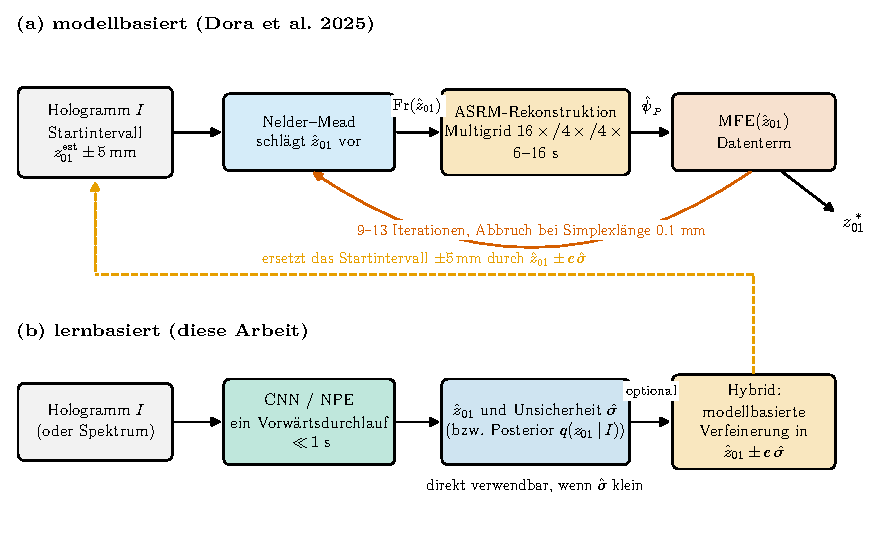
\includegraphics[width=\textwidth]{figures/stand_der_technik/autofokus_schema}
  \caption[Modellbasierter Autofokus und lernbasierte Schätzung im Vergleich]{%
    (a)~Geschachtelte Schleife des modellbasierten Autofokus nach
    \cite{dora2025autofocus}: Der Nelder--Mead-Optimierer schlägt einen Abstand
    $\hat z_{01}$ im Startintervall $z^{\mathrm{est}}_{01} \pm \qty{5}{\milli\metre}$
    vor, eine \ac{asrm}-Rekonstruktion mit der zugehörigen Fresnel-Zahl liefert
    die projizierte Welle $\hat\psi_P$, und der \ac{mfe} bewertet deren
    Konsistenz mit dem Hologramm. Bis zum Abbruch bei einer Simplexlänge von
    \qty{0.1}{\milli\metre} sind 9 bis 13 Rekonstruktionen zu je
    \qtyrange{6}{16}{\second} nötig. (b)~Lernbasierte Schätzung in dieser
    Arbeit: Ein Netz bildet das Hologramm (oder sein Leistungsspektrum) in einem
    Vorwärtsdurchlauf auf eine Schätzung mit Unsicherheit ab; diese ist entweder
    direkt verwendbar oder verengt als Startintervall die modellbasierte
    Verfeinerung (Hybrid).}
  \label{fig:stand:autofokus-schema}
\end{figure}

% ---------------------------------------------------------------------------
\begin{figure}[tb]
  \centering
  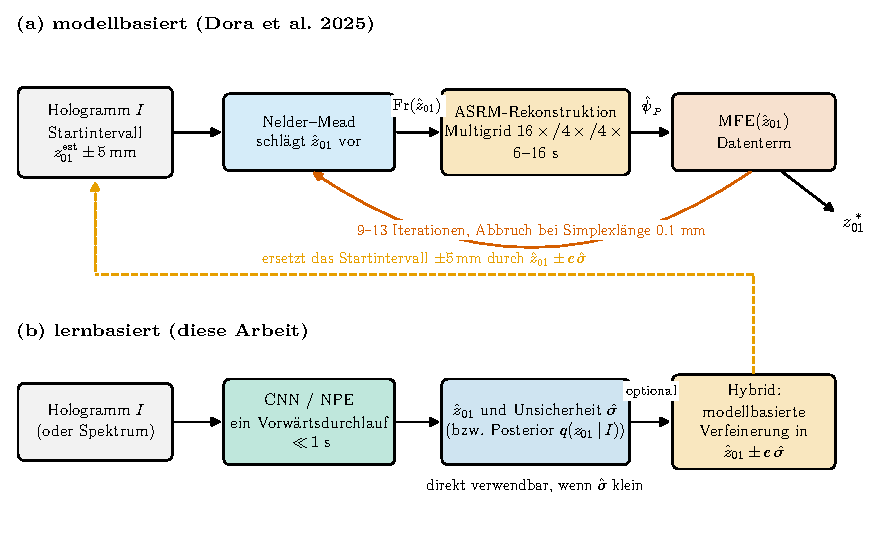
\includegraphics[width=\textwidth]{figures/stand_der_technik/autofokus_schema}
  \caption[Modellbasierter Autofokus und lernbasierte Schätzung im Vergleich]{%
    (a)~Geschachtelte Schleife des modellbasierten Autofokus nach
    \cite{dora2025autofocus}: Der Nelder--Mead-Optimierer schlägt einen Abstand
    $\hat z_{01}$ im Startintervall $z^{\mathrm{est}}_{01} \pm \qty{5}{\milli\metre}$
    vor, eine \ac{asrm}-Rekonstruktion mit der zugehörigen Fresnel-Zahl liefert
    die projizierte Welle $\hat\psi_P$, und der \ac{mfe} bewertet deren
    Konsistenz mit dem Hologramm. Bis zum Abbruch bei einer Simplexlänge von
    \qty{0.1}{\milli\metre} sind 9 bis 13 Rekonstruktionen zu je
    \qtyrange{6}{16}{\second} nötig. (b)~Lernbasierte Schätzung in dieser
    Arbeit: Ein Netz bildet das Hologramm (oder sein Leistungsspektrum) in einem
    Vorwärtsdurchlauf auf eine Schätzung mit Unsicherheit ab; diese ist entweder
    direkt verwendbar oder verengt als Startintervall die modellbasierte
    Verfeinerung (Hybrid).}
  \label{fig:stand:autofokus-schema}
\end{figure}

% ---------------------------------------------------------------------------
\begin{figure}[tb]
  \centering
  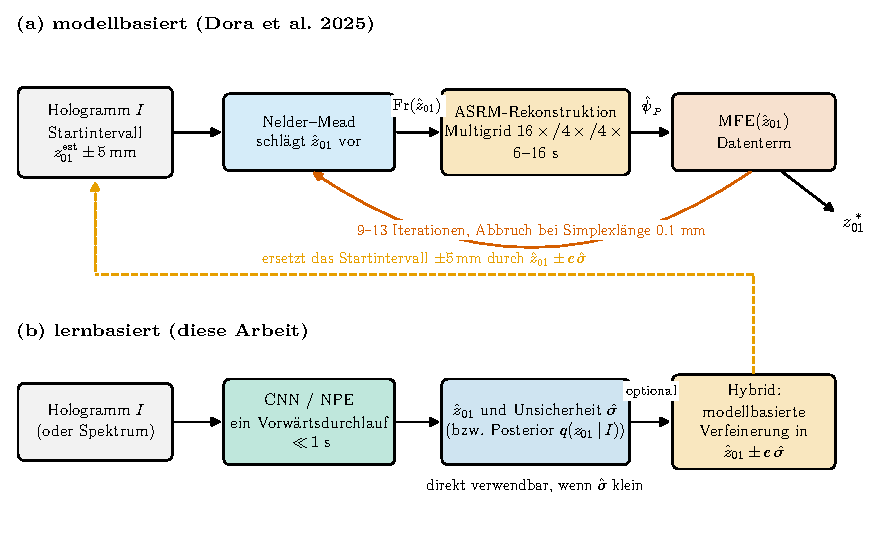
\includegraphics[width=\textwidth]{figures/stand_der_technik/autofokus_schema}
  \caption[Modellbasierter Autofokus und lernbasierte Schätzung im Vergleich]{%
    (a)~Geschachtelte Schleife des modellbasierten Autofokus nach
    \cite{dora2025autofocus}: Der Nelder--Mead-Optimierer schlägt einen Abstand
    $\hat z_{01}$ im Startintervall $z^{\mathrm{est}}_{01} \pm \qty{5}{\milli\metre}$
    vor, eine \ac{asrm}-Rekonstruktion mit der zugehörigen Fresnel-Zahl liefert
    die projizierte Welle $\hat\psi_P$, und der \ac{mfe} bewertet deren
    Konsistenz mit dem Hologramm. Bis zum Abbruch bei einer Simplexlänge von
    \qty{0.1}{\milli\metre} sind 9 bis 13 Rekonstruktionen zu je
    \qtyrange{6}{16}{\second} nötig. (b)~Lernbasierte Schätzung in dieser
    Arbeit: Ein Netz bildet das Hologramm (oder sein Leistungsspektrum) in einem
    Vorwärtsdurchlauf auf eine Schätzung mit Unsicherheit ab; diese ist entweder
    direkt verwendbar oder verengt als Startintervall die modellbasierte
    Verfeinerung (Hybrid).}
  \label{fig:stand:autofokus-schema}
\end{figure}

% ---------------------------------------------------------------------------
\begin{figure}[tb]
  \centering
  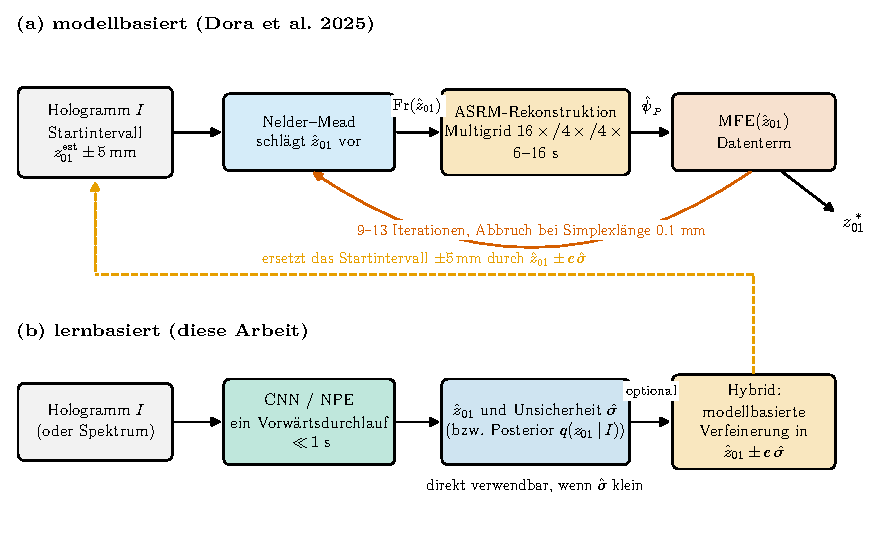
\includegraphics[width=\textwidth]{figures/stand_der_technik/autofokus_schema}
  \caption[Modellbasierter Autofokus und lernbasierte Schätzung im Vergleich]{%
    (a)~Geschachtelte Schleife des modellbasierten Autofokus nach
    \cite{dora2025autofocus}: Der Nelder--Mead-Optimierer schlägt einen Abstand
    $\hat z_{01}$ im Startintervall $z^{\mathrm{est}}_{01} \pm \qty{5}{\milli\metre}$
    vor, eine \ac{asrm}-Rekonstruktion mit der zugehörigen Fresnel-Zahl liefert
    die projizierte Welle $\hat\psi_P$, und der \ac{mfe} bewertet deren
    Konsistenz mit dem Hologramm. Bis zum Abbruch bei einer Simplexlänge von
    \qty{0.1}{\milli\metre} sind 9 bis 13 Rekonstruktionen zu je
    \qtyrange{6}{16}{\second} nötig. (b)~Lernbasierte Schätzung in dieser
    Arbeit: Ein Netz bildet das Hologramm (oder sein Leistungsspektrum) in einem
    Vorwärtsdurchlauf auf eine Schätzung mit Unsicherheit ab; diese ist entweder
    direkt verwendbar oder verengt als Startintervall die modellbasierte
    Verfeinerung (Hybrid).}
  \label{fig:stand:autofokus-schema}
\end{figure}
